\newpage
\section{Registro ore}
Nei seguenti paragrafi verrà spiegato come il gruppo intende dividere l'impegno dei ruoli nei cinque diversi periodi di sviluppo del software. All'ultimo paragrafo, verrà mostrato un riassunto con il totale del peso dei vari ruoli nell'intero progetto.

\subsection{Periodo di Analisi dei Requisiti}
Il primo periodo è l'\AdR. Esso non è rendicontabile ai fini di calcolo del preventivo, poichè non è da considerarsi a carico del committente. Le ore totali sono 189, suddivise come segue:

\begin{table}[H]
	\begin{center}
		\begin{tabular}{|c|c|c|}
			\hline
			\textbf{Ruolo}	& \textbf{Ore}	& \textbf{Ore remunerabili} \\
			\hline
			\Res	&	38	&  0 \\
			\hline
			\Amm	&	11	&  0 \\
			\hline
			\Ana	&	79	&  0 \\
			\hline
			\Ver	&	61	&  0 \\
			\hline
		\end{tabular}
	\end{center}
	\caption{Ore per ruolo, periodo di Analisi dei Requisiti}
\end{table}

L'incidenza di tali ore determina in percentuale come mostrato di seguito:
\begin{figure}[H]
	\centering
	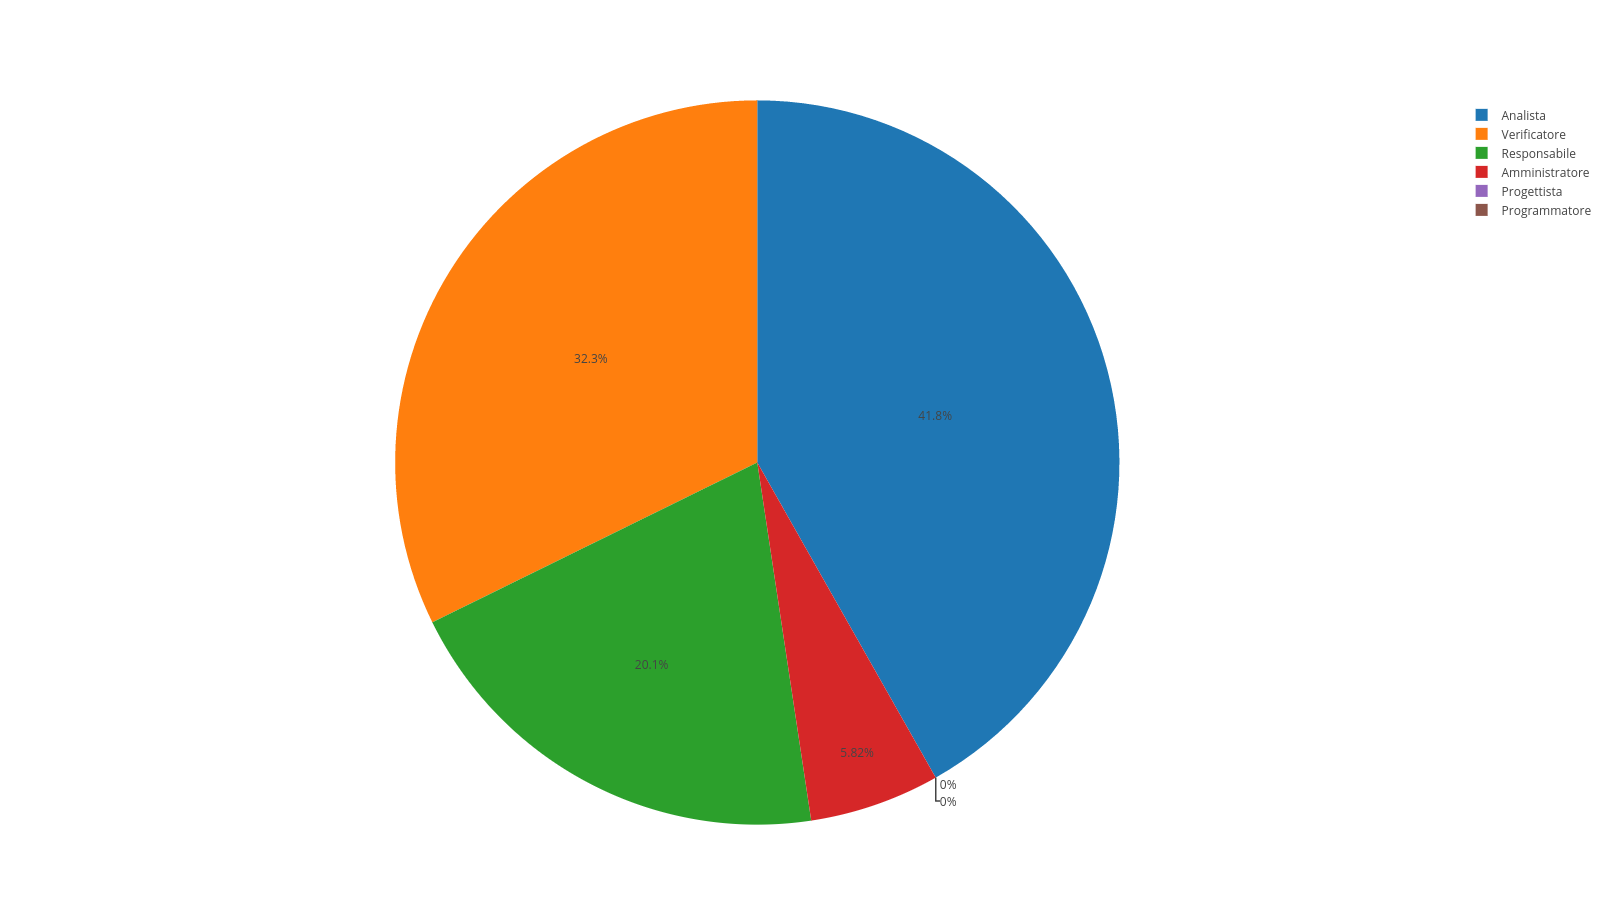
\includegraphics[scale=0.6]{img/AnalisiRequisiiti.png}
	\caption{Incidenza ore per ruolo, periodo di Analisi dei Requisiti}
\end{figure}

\subsection{Periodo di Analisi dei Requisiti Dettagliata}
La seconda porzione di Analisi dei Requisiti, da svolgersi dopo la Revisione dei Requisiti, è l'Analisi dei Requisiti Dettagliata. Come per il precedente, esso è da considerarsi parte dell'investimento intrapreso e quindi non è rendicontabile ai fini di calcolo del preventivo. Le ore totali sono 15, suddivise come segue:

\begin{table}[H]
	\begin{center}
		\begin{tabular}{|c|c|c|}
			\hline
			\textbf{Ruolo}	& \textbf{Ore}	& \textbf{Ore remunerabili} \\
			\hline
			\Res	&   4 	&  0  \\
			\hline
			\Amm	&   1	&  0	\\
			\hline
			\Ana	&   5	&  0	\\
			\hline
			\Ver	&   5	&  0	\\
			\hline
		\end{tabular}
	\end{center}
	\caption{Ore per ruolo, periodo di Analisi dei Requisiti}
\end{table}

L'incidenza di tali ore determina in percentuale come mostrato di seguito:
\begin{figure}[H]
	\centering
	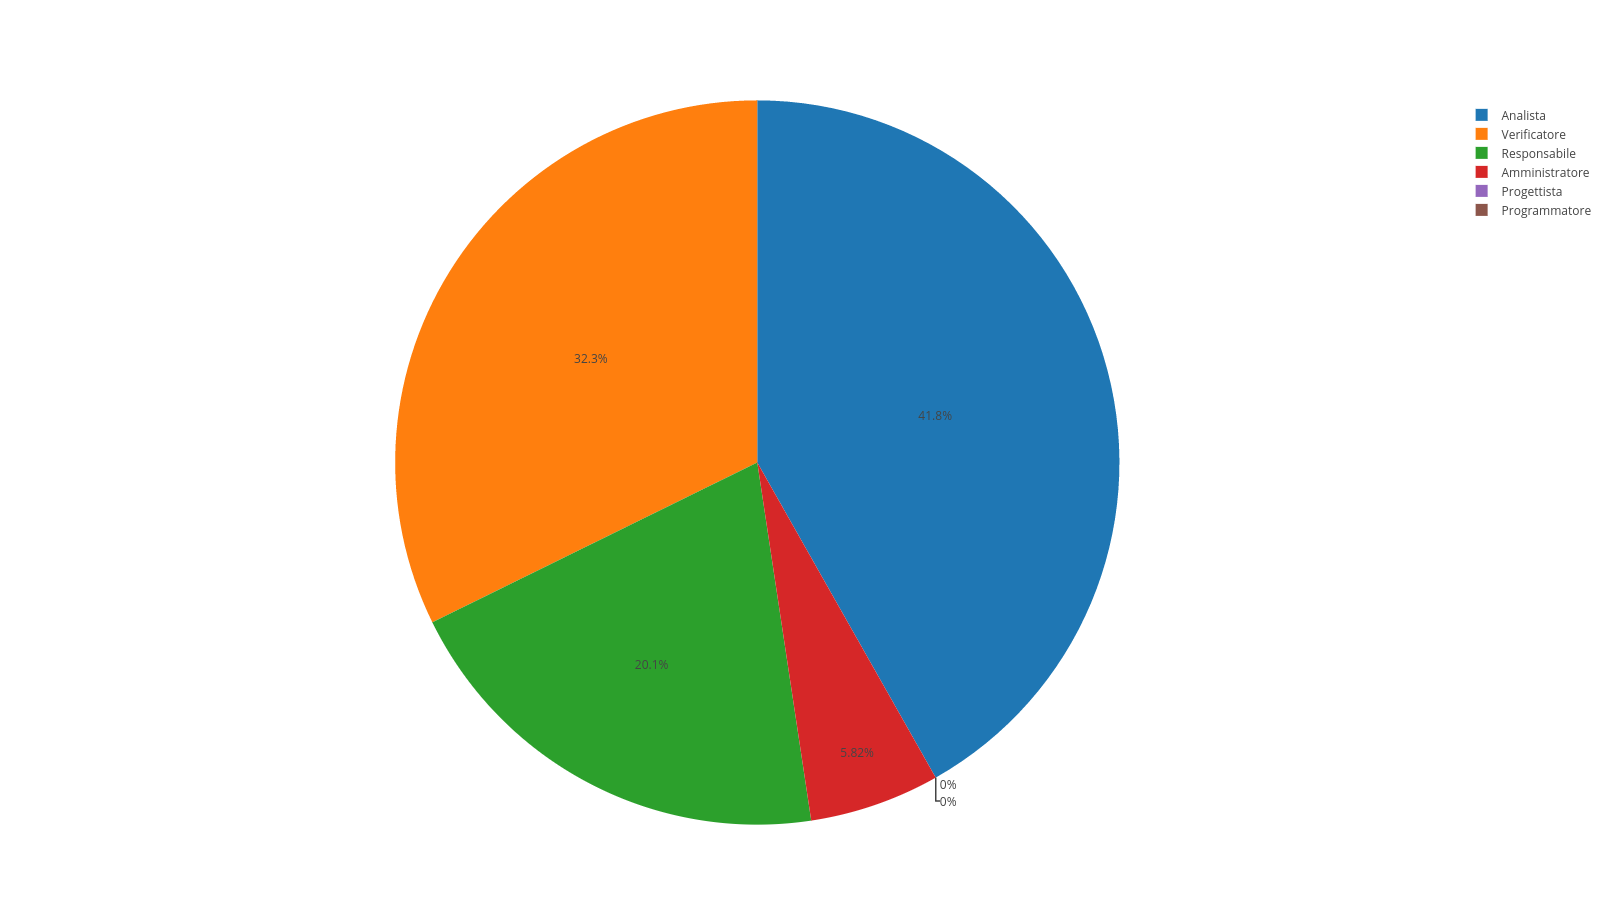
\includegraphics[scale=0.6]{img/AnalisiRequisiiti.png}
	\caption{Incidenza ore per ruolo, periodo di Analisi dei Requisiti}
\end{figure}

\subsection{Periodo di Progettazione Architetturale}
Lo sviluppo procede con la Progettazione Architetturale. Le ore totali sono 200, suddivise come segue:

\begin{table}[H]
	\begin{center}
		\begin{tabular}{|c|c|c|}
			\hline
			\textbf{Ruolo}	& \textbf{Ore}	& \textbf{Ore remunerabili} \\
			\hline
			\Res	&	5	&	5	\\
			\hline
			\Amm	&	5	&	5	\\
			\hline
			\Prog   &	138   &	138	\\
			\hline
			\Ver	&	52	&	52	\\
			\hline
		\end{tabular}
	\end{center}
	\caption{Ore per ruolo, periodo di Progettazione Architetturale}
\end{table}

L'incidenza di tali ore determina in percentuale come mostrato di seguito:
\begin{figure}[H]
	\centering
	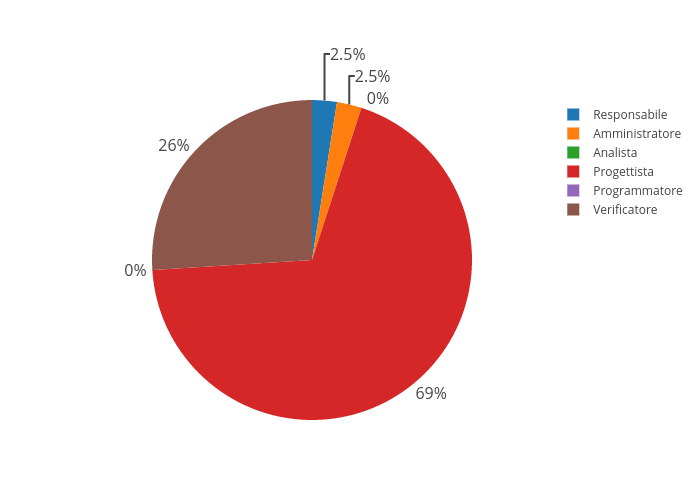
\includegraphics[scale=0.6]{img/ProgettazioneArchitetturale.png}
	\caption{Incidenza ore per ruolo, periodo di Progettazione Architetturale}
\end{figure}

\subsection{Periodo di Progettazione Architetturale Dettagliata}
Il terzo periodo è la Progettazione Architetturale Dettagliata. Le ore totali sono 118, suddivise come segue:

\begin{table}[H]
	\begin{center}
		\begin{tabular}{|c|c|c|}
			\hline
			\textbf{Ruolo}	& \textbf{Ore}	& \textbf{Ore remunerabili} \\
			\hline
			\Res	&	5	&	5 \\
			\hline
			\Amm	&	6	&	6	\\
			\hline
			\Prog   &	72   &	72	\\
			\hline
			\Ver	&	35	&	35	\\
			\hline
		\end{tabular}
	\end{center}
	\caption{Ore per ruolo, periodo di Progettazione Architetturale Dettagliata}
\end{table}

L'incidenza di tali ore determina in percentuale come mostrato di seguito:
\begin{figure}[H]
	\centering
	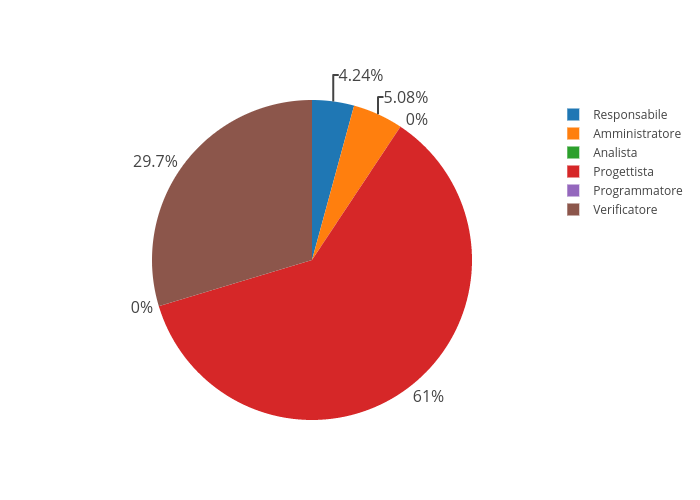
\includegraphics[scale=0.6]{img/ProgettazioneDettaglio.png}
	\caption{Incidenza ore per ruolo, periodo di Progettazione Architetturale Dettagliata}
\end{figure}

\subsection{Periodo di Codifica}
Il penultimo periodo è la Codifica. Le ore totali sono 213, suddivise come segue:

\begin{table}[H]
	\begin{center}
		\begin{tabular}{|c|c|c|}
			\hline
			\textbf{Ruolo}	& \textbf{Ore}	& \textbf{Ore remunerabili} \\
			\hline
			\Res	&	6	&	6	\\
			\hline
			\Amm	&	3	&	3	\\
			\hline
			\Progr   &	143   &	143	\\
			\hline
			\Ver	&	61	&	61	\\
			\hline
		\end{tabular}
	\end{center}
	\caption{Ore per ruolo, periodo di Codifica}
\end{table}

L'incidenza di tali ore determina in percentuale come mostrato di seguito:
\begin{figure}[H]
	\centering
	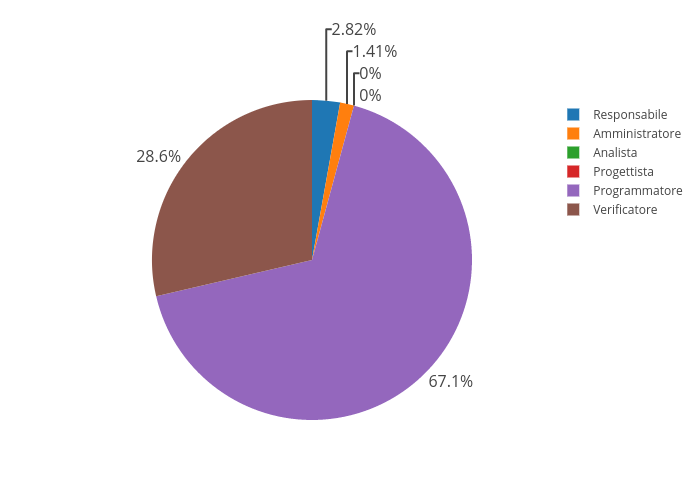
\includegraphics[scale=0.6]{img/Codifica.png}
	\caption{Incidenza ore per ruolo, periodo di Codifica}
\end{figure}

\subsection{Periodo di Verifica e Validazione}
L'ultimo periodo è la Verifica del prodotto sviluppato. Le ore totali sono 99, suddivise come segue:

\begin{table}[H]
	\begin{center}
		\begin{tabular}{|c|c|c|}
			\hline
			\textbf{Ruolo}	& \textbf{Ore}	& \textbf{Ore remunerabili} \\
			\hline
			\Res	&	3  &	3	\\
			\hline
			\Amm	&	3  &	3	\\
			\hline
			\Prog   &	15  &	15	\\
			\hline
			\Ver	&	78	&	78	\\
			\hline
		\end{tabular}
	\end{center}
	\caption{Ore per ruolo, periodo di Verifica e Validazione}
\end{table}

L'incidenza di tali ore determina in percentuale come mostrato di seguito:
\begin{figure}[H]
	\centering
	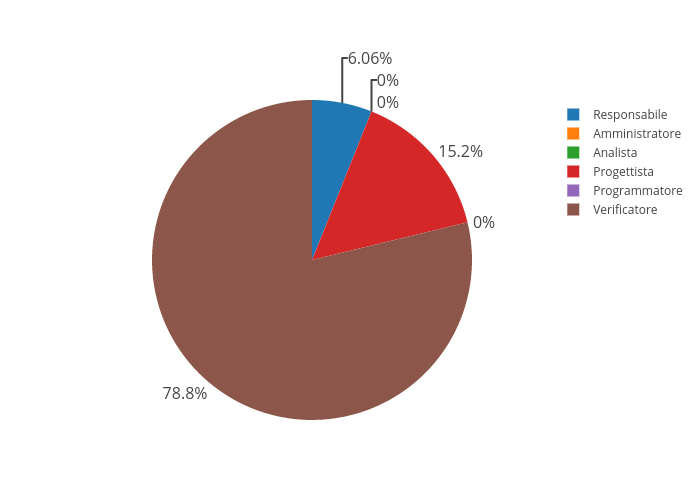
\includegraphics[scale=0.6]{img/Validazione.png}
	\caption{Suddivisione ore per ruolo, periodo di Verifica e Validazione}
\end{figure}

\subsection{Riepilogo}
Le ore totali del necessarie allo sviluppo sono 837 di cui, scorporando la fase di Analisi dei Requisiti, 630 remunerabili. Complessivamente le ore sono suddivise come segue:

\begin{table}[H]
	\begin{center}
		\begin{tabular}{|c|c|c|}
			\hline
			\textbf{Ruolo}	& \textbf{Ore complessive} & \textbf{Ore remunerabili} \\
			\hline
			\Res	&	61	&	19	\\
			\hline
			\Amm	&	30	&	17	\\
			\hline
			\Ana	&	84	&	0	\\
			\hline
			\Prog	&	225	&	225	\\
			\hline
			\Progr	&	143	&	143	\\
			\hline
			\Ver	&	294	&	226	\\
			\hline
		\end{tabular}
	\end{center}
	\caption{Ore per ruolo, Riepilogo}
\end{table}

L'incidenza di tali ore incide in percentuale come mostrato di seguito, prima complessive e poi remunerative:
\begin{figure}[H]
	\centering
	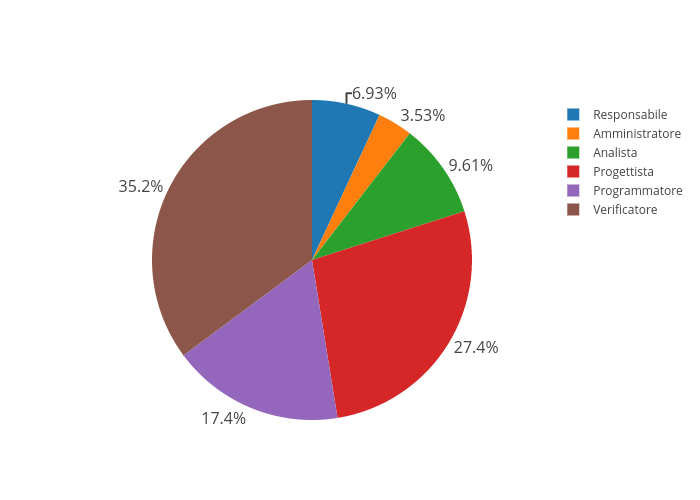
\includegraphics[scale=0.6]{img/OreTotali.png}
	\caption{Suddivisione ore per ruolo, riepilogo totale}
\end{figure}
\begin{figure}[H]
	\centering
	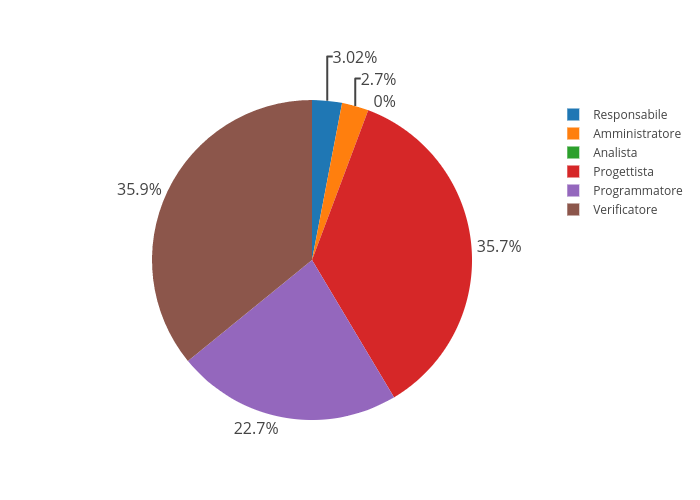
\includegraphics[scale=0.6]{img/OreRendicontabili.png}
	\caption{Suddivisione ore per ruolo, riepilogo ore remunerabili}
\end{figure}

